% Document class
% Document class
% chktex-file 44
% chktex-file 13
% chktex-file 8
\documentclass[12pt,a4paper]{article}%

% Packages
\usepackage[utf8]{inputenc}%
\usepackage[T1]{fontenc}%
\usepackage{indentfirst}%
\usepackage{geometry}%
\usepackage{setspace}%
\usepackage{times}%
\usepackage{lipsum}% For dummy text
\usepackage{graphicx}%
\usepackage{fancyhdr}%
\usepackage{titlesec}%
\usepackage{tocloft}%
\usepackage{amsmath,amssymb}%
\usepackage{caption}%
\usepackage{subcaption}%
\usepackage{booktabs}%
\usepackage{hyperref}%
\usepackage{natbib}%
\usepackage{float}
% Geometry
\geometry{
  a4paper,
  left=3cm,
  right=2cm,
  top=2cm,
  bottom=2cm
}%

% Line spacing
\onehalfspacing%

% Page numbering
\pagestyle{fancy}%
\fancyhf{}%
\rfoot{\thepage}%

% Section formatting
\titleformat{\section}[block]{\normalfont\Large\bfseries}{\thesection}{1em}{}%
\titleformat{\subsection}[block]{\normalfont\large\bfseries}{\thesubsection}{1em}{}%

% Table of contents formatting
\renewcommand{\cftsecleader}{\cftdotfill{\cftdotsep}}%

% Paragraph formatting
\setlength{\parindent}{1.25em} % Indent for ALL paragraphs, including first
\setlength{\parskip}{0em}      % No extra spacing between paragraphs

\begin{document}

\section{Responsibility for Household Carbon Emissions}
\subsection{Rethinking Responsibility}

Households are often portrayed as central actors in climate mitigation—urged to fly less, retrofit their homes, shift their diets, or reduce electricity use. Yet, the basis on which such responsibility is assigned remains contested. What does it mean to hold a household responsible for climate change, and how do we ensure that this responsibility is fair, actionable, and grounded in reality?

Existing carbon accounting methods offer different answers. Some emphasize direct control over emissions, others focus on consumption or supply chains, and still others ask whether a household’s actions actually reduce emissions. These differences reflect deeper questions about agency, influence, and obligation. 

This chapter rethinks household responsibility by comparing the attribution logics embedded in four key models—production-based (GHG Protocol), product-based (LCA), demand-based (EEIO), and marginal impact models (Hakenes and Schliephake) \footnote{The Hakenes and Schliephake model can be understood as a general equilibrium carbon footprint model, as it determines household responsibility based on the marginal change in total emissions across interconnected markets resulting from a behavioral shift, accounting for substitution, spillovers, and price effects.}. Our aim is to evaluate not only how these methods measure emissions, but also how they construct the idea of responsibility itself and with what consequences for policy, fairness, and climate action.

\subsection{Attribution Principles}

\subsubsection{Attribution Based on Operational Control}

Control-based attribution allocates emissions to the actor who directly controls the physical source of greenhouse gas release. Emissions are assigned based on \textit{operational responsibility},that is, who manages the combustion process or industrial activity rather than on who benefits from or demands the resulting goods and services. In this framework, emissions from electricity generation are attributed to power plants, and those from food or goods production are attributed to manufacturing firms, not to the households that consume the outputs.

The GHG Protocol is the principal framework that operationalizes this logic. In household-level applications, it typically attributes emissions only from direct fuel use (e.g., home heating, personal vehicles) and from purchased electricity or heat (Scopes 1 and 2). Emissions embedded in goods, services, or infrastructure (commonly classified as Scope 3) are excluded unless separately modeled. As a result, household responsibility appears significantly lower than in consumption-based frameworks. For instance, while households in developed economies are responsible for an estimated 60–70\% of emissions under a consumption-based approach, control-based inventories typically attribute only 10–20\% to them.\footnote{See Hertwich and Peters (2009). Consumption-based GHG emissions. \textit{Environmental Science \& Technology}.}

This method reflects a production-based understanding of responsibility: households are held accountable for emissions they physically generate or for energy they purchase, but not for upstream emissions embodied in their consumption. Although narrower in scope, this attribution style serves a clear regulatory function. Its operational clarity makes it particularly suitable for emissions inventories, carbon pricing schemes, and supply-side decarbonization policies that target industrial emitters rather than individuals. The GHG Protocol underpins most national reporting systems and corporate disclosures, and is explicitly aligned with policy instruments such as emissions caps, sectoral mitigation targets, and producer-level carbon accounting.\footnote{See World Resources Institute and WBCSD (2004). \textit{The Greenhouse Gas Protocol: A Corporate Accounting and Reporting Standard}. Also see den Elzen et al. (2020), \textit{Nature Climate Change}, on policy alignment of production-based accounting.} By tracing emissions to producers rather than consumers, control-based attribution enables system-level mitigation efforts without requiring detailed behavioral data at the household level.

\subsubsection{Consumption-Based Attribution}

Consumption-based attribution assigns responsibility for emissions to end users, based on the idea that consumer demand drives production and, ultimately, greenhouse gas emissions. Unlike control-based methods that assign emissions to producers, consumption-based frameworks trace emissions along the supply chain and allocate them to the final household that purchases or uses the good or service.

Among the methods reviewed in this paper, two approaches operationalize consumption-based attribution: life cycle assessment (LCA) and environmentally extended input–output (EEIO) models. Both assign emissions to households for the upstream impacts of their consumption, but they differ in analytical resolution and system boundaries. LCA focuses on product-level analysis by quantifying emissions over a product’s entire life cycle—from raw material extraction through use and disposal.\footnote{Curran, M. A. (2015). Life Cycle Assessment: Principles and Practice. EPA.} This method enables fine-grained comparisons of consumption choices (e.g., meat versus plant-based diets) and supports interventions like eco-labeling and sustainable procurement.

EEIO models, by contrast, estimate emissions based on monetary flows across sectors and are designed to capture systemic effects across entire economies. They link household expenditure data with environmental accounts using national input–output tables, assigning emissions in proportion to spending across categories such as food, transport, and housing.\footnote{Wiedmann, T. (2009). A review of recent multi-region input–output models used for consumption-based emission accounting. \textit{Ecological Economics}.} While LCA relies on detailed process-level data, EEIO models are structured around macroeconomic datasets, making them suitable for national-scale analysis and policy evaluation.

Both approaches consistently attribute a large share of global emissions to households, typically between 60\% and 70\% in high-income countries, by including indirect emissions embedded in consumption.\footnote{Ivanova, D. et al. (2016). Environmental impact assessment of household consumption. \textit{Journal of Industrial Ecology}.} This high attribution has made consumption-based methods influential in shaping narratives around individual climate responsibility and has informed the design of tools such as carbon footprint calculators, dietary guidelines, and voluntary offsetting schemes. However, these methods also risk overstating household agency by abstracting from structural constraints, supply-side inertia, and the availability of low-carbon alternatives.

Despite these limitations, consumption-based attribution provides valuable insights for policymaking. It highlights carbon-intensive lifestyle domains, supports the development of behavioral nudges and fiscal instruments (e.g., carbon taxes or subsidies), and enables differentiated climate strategies across income groups. In this way, it complements production-based models by identifying downstream leverage points for demand-side mitigation.

\subsubsection{Consequentialist Attribution}

The general equilibrium structure and derivation of the Hakenes and Schliephake (2024) model are presented in Chapter~7. Here, we focus specifically on how the model attributes responsibility for emissions—offering a fundamentally different logic from control- or consumption-based methods.

Consequentialist attribution links household responsibility to the actual change in total emissions resulting from marginal economic decisions. In contrast to attribution by operational control or average consumption, this approach estimates how much aggregate emissions would differ if a household were absent from the economy. The household’s carbon footprint is thus defined as the causal marginal impact of its consumption and investment choices on total emissions.

Within the Hakenes–Schliephake framework, emissions are attributed through a counterfactual comparison: the general equilibrium of the full economy versus the equilibrium that would occur if a given household did not participate. Because the model includes both product and financial markets, the resulting footprint incorporates not only direct effects but also indirect spillovers through price mechanisms, risk-adjusted investments, and inter-household substitution. The marginal impact of a household’s behavior is calculated using a weighting parameter, $\varphi$, which determines the relative attribution of emissions between consumption and investment.\footnote{Hakenes, H. \& Schliephake, E. (2024). Your Carbon Footprint, Including Investments. SSRN 4710536. See also Section~7.1.4 in this thesis for derivation of $\varphi$.}

This weighting is sensitive to structural characteristics of the economy: greater risk aversion or financial volatility shifts responsibility toward consumption, while higher substitutability across sectors amplifies the spillover effect through investment. As a result, households are only held responsible for emissions they can meaningfully influence. If consumption is perfectly substitutable or investment flows are fully absorbed by other agents, the attributed footprint may approach zero—even if the household’s nominal expenditure is large.

By assigning responsibility based on marginal system-wide impact, the model avoids double-counting and mitigates the over-attribution seen in static frameworks. It also aligns well with policy approaches that emphasize structural levers, such as green financial regulation or carbon-intensity weighting of investment portfolios. While less intuitive and more data-intensive than other methods, this attribution logic provides a refined lens for distinguishing symbolic from substantive household climate action.

\subsection{Comparative Synthesis of Attribution Frameworks}

Attribution methods differ not only in analytical structure but in how they frame responsibility—what they assign to households, what they assume about agency, and what they ignore. As visualized in Figure~\ref{fig:heatmap}, these differences create meaningful trade-offs that shape both interpretation and policy relevance.

Control-based attribution (GHG Protocol) limits household responsibility to direct actions, minimizing the risk of over-attribution but offering little behavioral or structural insight. Consumption-based approaches (LCA and EEIO) invert this: they assign large shares of emissions to households, enabling lifestyle-oriented analysis but often abstracting from real-world constraints, rebound effects, or structural inertia. They perform well descriptively but struggle to differentiate between symbolic and effective action.

Only the Hakenes and Schliephake model formally incorporates systemic feedbacks. Its consequentialist logic reframes attribution as marginal influence, not average burden. This avoids double-counting and grounds responsibility in causal agency, but at the cost of complexity, abstraction, and limited communicability.

Figure~\ref{fig:heatmap} illustrates this spectrum: methods differ in how much they reveal about behavioral influence, how they treat economic structure, and how carefully they delimit the scope of household responsibility. Choosing an attribution framework is therefore not just a technical exercise—it reflects underlying assumptions about fairness, tractability, and what forms of action are worth encouraging.

\begin{figure}[H]
    \centering
    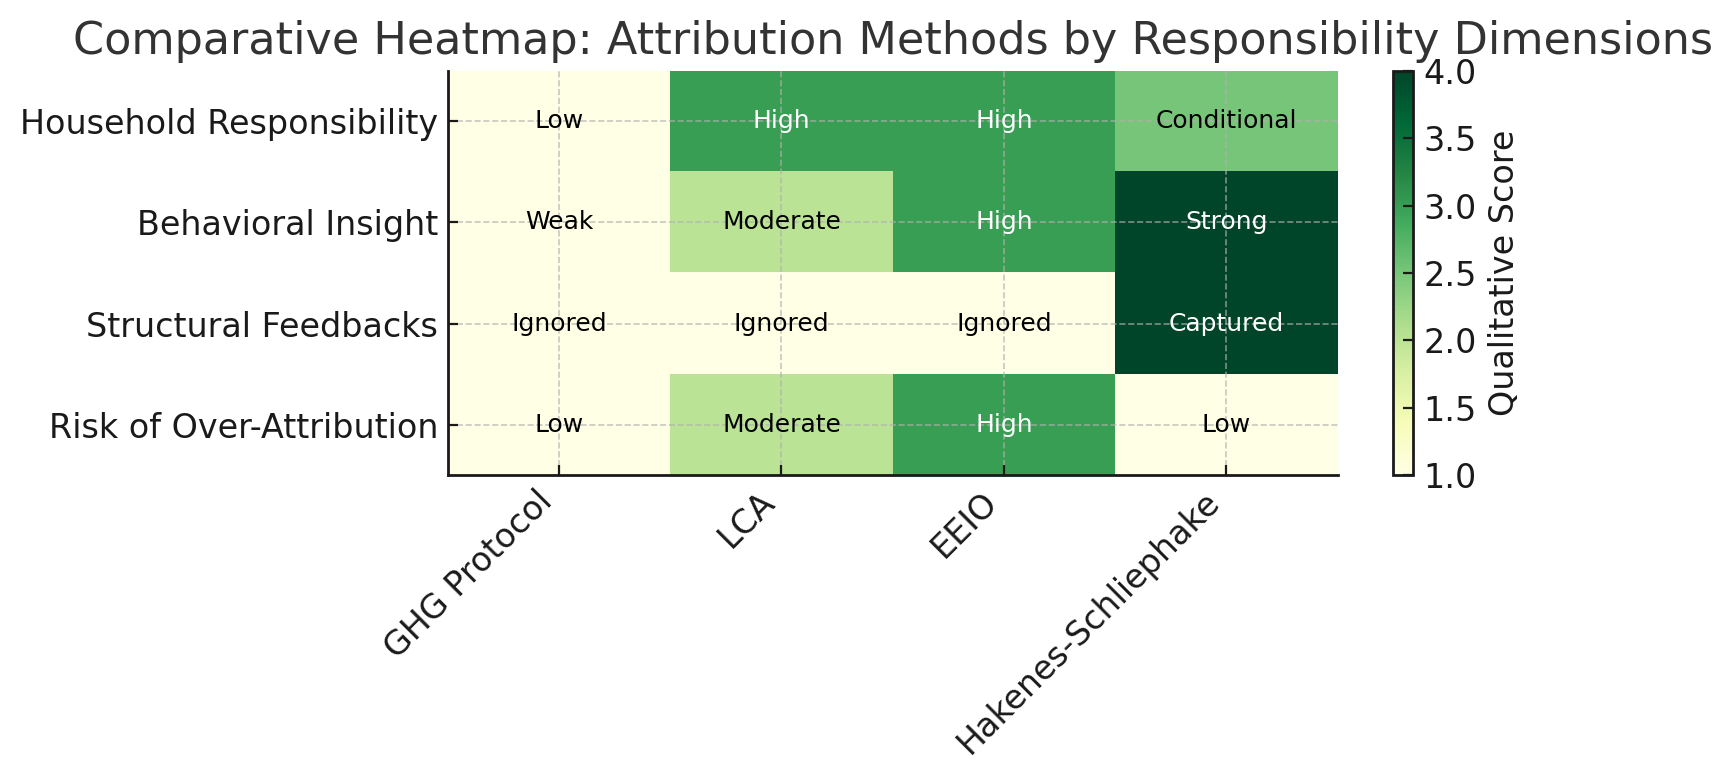
\includegraphics[width=\textwidth]{attribution_heatmap.png}
    \caption{Comparative heatmap of attribution frameworks across key responsibility dimensions. Higher scores indicate greater behavioral relevance, structural sensitivity, or risk of over-attribution. Source: Author's own analysis based on Hertwich and Peters (2009), Ivanova et al. (2016), Hakenes and Schliephake (2024), and Capstick et al. (2019).}
    \label{fig:heatmap}
\end{figure}

\noindent
This synthesis sets the stage for the next chapter, where we assess how different attribution logics align with climate policy instruments and what this implies for equitable mitigation strategies.

\end{document}